
% LP: copie de l'intro de Xavier
In NIKA2, the opacity is measured via a total-power technique, which was successfully tested with NIKA. The details of this technique and its agreement with the Atmospheric Transmission at Microwaves (ATM) model (\cite{2001IEEE....49.1683C}) are described in \cite{Catalano:2014nml}. The underlying idea is to replace the opacity, usually delivered by the resident IRAM tau-meter that performs elevation scans at a fixed azimuth and is operating at 225\,GHz, by a measurement that uses the NIKA2 instrument itself as a tau-meter. Using this procedure we can directly derive an opacity integrated in the NIKA2 very bandpasses and in the same line-of-sight of the source in the considered map. First, we have to calibrate the relationship between total power and opacity.
% fin copie

\subsection{Methodology}
For each kid $k$, the absolute value of the resonance frequency
$f_{tone}^k$ moves with the atmospheric load according to

\begin{equation}
f_{tone}^k = C_0^k + C_1^k T_{atm}[1-e^{-\tau/\sin\delta}]
\end{equation}

{\bf LP: pourquoi signe plus alors qu'on utilise un signe moins dans
  Eq. 2 du papier instru ?}

where $C_0^k$ is a constant equal to the resonance
frequency at zero opacity, $C_1^k$ is the calibration conversion
factor in kHz$/$K, $T_{atm}$ is the equivalent temperature
of the atmosphere (taken as a constant at 270K), $\tau$ the zenith
opacity and $\delta$ the average elevation of the telescope.
By assuming a homogeneous plane-parallel atmosphere, the airmass $x$ is defined from the
elevation as $x = \sin\delta$. 

The coefficients $C_0^k$ and $C_1^k$ are expected to be constant in time
within at least a cooldown cycle, and are determined using a {\tt
  skydip} procedure. This consists in moving
the telescope in elevation step by step and to monitor, for each kid, the
evolution of $f_{tone}^k$ versus the air mass and to fit the zenith opacity $\tau$ and
$C_0^k$ and $C_1^k$. During a {\tt skydip}, the telescope performs
eleven  steps in the elevation range from 19 to 65 degrees, regularly
spaced in airmass. For each step, we acquire about twenty seconds of
time traces to reduce the error in the determination of $f_{tone}^k$.

All skydips, obtained under various opacity
conditions, are analysed together to break the degeneracies between
the opacity and the responsivity. The procedure has two steps.
First, all the skydips are analysed individually to simply measure
$f_{tone}^k$ for each stable elevation and fit simultaneously all 
parameters ($\tau$, $C_0^k$ and $C_1^k$.)
Error bars on $\tau$ are estimated by doing
this procedure on blocks of 40 kids only and getting a dispersion on the
resulting $\tau$ from the different blocks. Usually the dispersion comes out as
$4\times 10^{-3}$ at 1mm and $1\times 10^{-3}$ at 2mm. Once the $\tau$ values
are estimated for each skydip (as the average over the blocks), we compute
(while fixing $\tau$) the $C_0$ and $C_1$ final values for each KID. We thus
retrieve the coefficients of all the KIDs even though some of them could not
contribute to the tau determination.

%% \begin{figure}
%% \begin{center}
%% 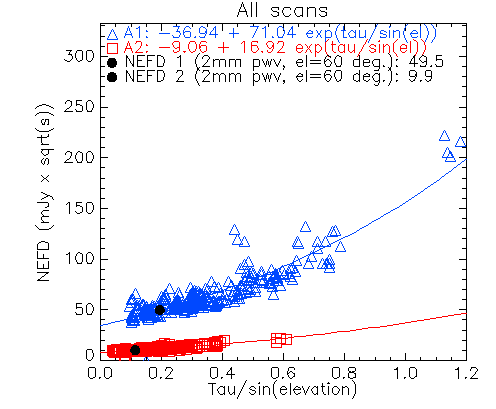
\includegraphics[clip, angle=0, scale =
%%   0.5]{Figures/NEFD_vs_tau_20170226s415_FXDC0C1_Jy_common_mode_kids_out.png}
%% 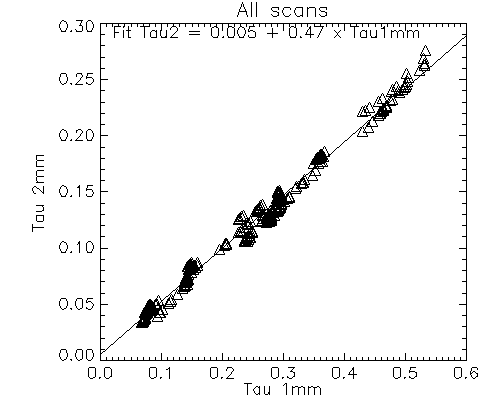
\includegraphics[clip, angle=0, scale =
%%   0.5]{Figures/tau1_tau2_20170226s415_FXDC0C1_GaussPhot_common_mode_kids_out.png}
%% \caption{}
%% \label{fig:fov}
%% \end{center}
%% \end{figure}

%  figure deplacee dans Opacity_checks.tex
%\begin{figure}
%\begin{center}
%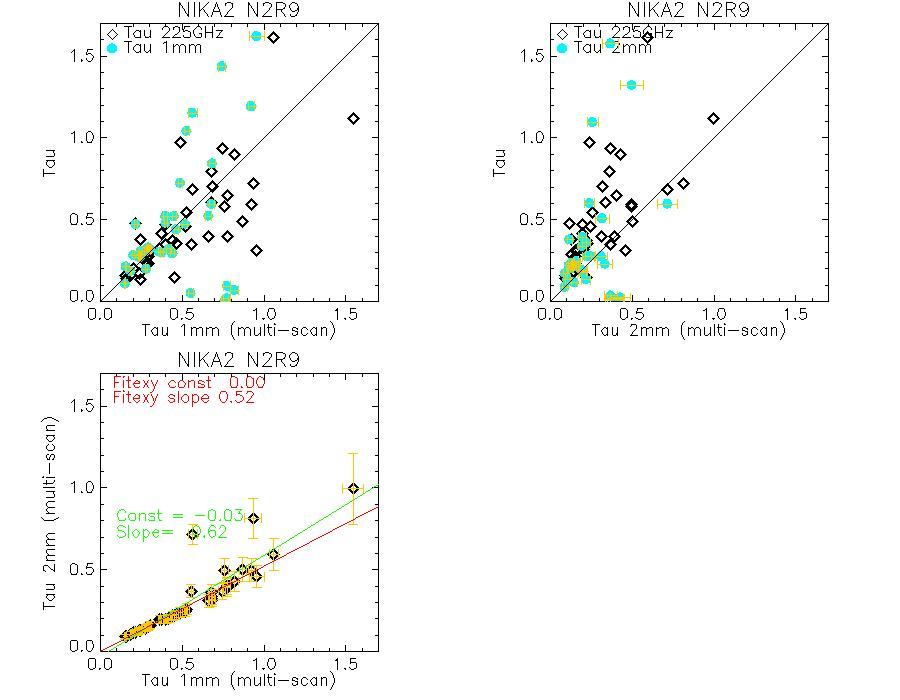
\includegraphics[clip, angle=0, scale = 0.5]{Figures/test_allskd_N2R9.jpg}
%\caption{{\bf Fix me : improve plot quality and plot only the 3rd one.}}
%\label{fig:test_allskd_N2R9}
%\end{center}
%\end{figure}
